\documentclass[letterpaper,10pt]{article}
\usepackage[top=2cm, bottom=1.5cm, left=1cm, right=1cm]{geometry}
\usepackage{amsmath, amssymb, amsthm,graphicx}
\usepackage{fancyhdr}
\pagestyle{fancy}

\lhead{\today}
\chead{Quality Engineering Assignment 5}
\rhead{Justin Hood}

\newcommand{\Z}{\mathbb{Z}}
\newcommand{\Q}{\mathbb{Q}}
\newcommand{\R}{\mathbb{R}}
\newcommand{\C}{\mathbb{C}}
\newtheorem{lem}{Lemma}

\begin{document}
\begin{enumerate}
\item The sample of inside diameters of bearings in aircraft landing gears has,
\[\mu=8.2535,\ \sigma=0.002\]
We shall construct a hypothesis test to see whether the true mean is \[\mu=8.25\]
This is a two sided test. The hypotheses are,
\[H_0: \mu=8.25,\ \ \ H_A: \mu \neq 8.25\]
First, we compute the test statistic as,
\[Z^*=\frac{\bar{x}-\mu}{\sigma/\sqrt{n}}=\frac{8.2535-8.25}{0.002/\sqrt{15}}\approx 6.77772\]
We note that the critical value for an $\alpha=0.05$ test is $Z_C=1.959964$. Here, we see that our computed test statistic is far above this threshold. So, we shall reject the null hypothesis, that $\mu=8.25$ in favor of the alternative hypothesis, that $\mu\neq 8.25$.
\item The tensile strength of a fiber for manufacturing has,
\[\mu=127,\ \sigma=2\]
We shall construct a hypothesis test to see whether the following hypothesis:
\[H_0: \mu=125,\ \ \ H_A: \mu > 125\]
This is a one sided test, and the statistic is computed as follows:
\[Z^*=\frac{\bar{x}-\mu}{\sigma/\sqrt{n}}=\frac{127-125}{2/\sqrt{8}}\approx 2.82843\]
The critical value with $\alpha=0.05$ is $Z_c=1.64485$. Here, we clearly see that the computed statistic is larger than the critical value. Thus, we shall reject the null hypothesis, that the mean is $\mu=125$ in favor of the alternative, that the mean is $\mu >125$.
\item We consider now, the service life of a battery in pacemakers. A random sample of 10 batteries is run continuously and the following data obtained:
\[x=(25.5, 26.1, 26.8, 23.2, 24.2, 28.4, 25.0, 27.8, 27.3, 25.7)\]
Using MiniTab, we compute the follwing:
\[\mu_x=26,\ \ s_x=1.62481\]
We shall now test the following hypothesis,
\[H_0: \mu<= 25,\ \ \ H_A: \mu>25\]
Our test statistic is then,
\[t^*=\frac{\bar{x}-\mu}{s/\sqrt{n}}=\frac{26-25}{1.62481/\sqrt{10}}\approx 1.946244583\]
For a one sample $t$ test with $\alpha=0.05$, we see that the critical value is $t_C=1.8331$. Here, our calculated test statistic is greater, thus, we shall reject the null hypothesis that $\mu<=25$ in favor of the alternative hypothesis that $\mu>25$. Thus, at the $\alpha=0.05$ level, the manufacturer may conclude that the mean life exceeds 25 hours as desired.
\item We consider two different soft drink bottling machines, with associated data,
\begin{align*}
\sigma_1=0.010\ \ \ \ \ &\sigma_2=0.015\\
n_1=25\ \ \ \ \ &n_2=20\\
\bar{x}_1=2.04\ \ \ \ \ &\bar{x}_2=2.07
\end{align*}
We shall test the following:
\[H_0: \mu_1=\mu_2,\ \ \ H_A: \mu_1 \neq \mu_2\]
We perform a two sample $z$ test and obtain the following statistic,
\[Z^*=\frac{\bar{x}_1-\bar{x}_2}{\sqrt{\frac{\sigma_1^2}{n_1}+\frac{\sigma_2^2}{n_2}}}=\frac{2.04-2.07}{\sqrt{\frac{.01^2}{25}+\frac{.015^2}{20}}}\approx -7.682213\]
For this $z$ test with $\alpha=0.05$, the critical z value is $|Z_C|=1.95996$. Here, we see that our value is clearly greater. Thus, we shall reject the null hypothesis, that $\mu_1=\mu_2$ in favor of the alternative that $\mu_1\neq \mu_2$.
\item We consider two processes for quenching on a metal alloy, saltwater and oil. Assuming normality in hardness, we consider the data provided. Using Excel, we are able to compute,
\begin{center}
\begin{tabular}{|c||c|c|}
\hline
& SaltWater & Oil \\\hline
$\bar{x}$ & 147.6 & 149.4\\\hline
$Var$ & 24.71111 & 29.82222\\\hline
$StdDev$ & 4.971027 & 5.460973\\\hline
\end{tabular}
\end{center}
For the two samples. We now consider the hypotheses,
\[H_0: \mu_{SW}=\mu_O,\ \ \ H_A: \mu_{SW} \neq \mu_O\]
We note that the sample standard deviations are similar, so we shall use a pooled $t$ test to compare the means. First, we compute the pooled standard deviation as,
\begin{align*}
s_P&=\sqrt{\frac{(n_1-1)s_1^2+(n_2-1)s_2^2}{n_1+n_2-2}}\\
&=\sqrt{\frac{(10-1)24.71111+(10-1)29.82222}{10+10-2}}\\
&=\sqrt{27.26666}\\
&\approx 5.22175
\end{align*}
We can now compute the $t$ statistic as,
\[t^*=\frac{\bar{x}_{SW}-\bar{x}_O}{s_P/\sqrt{\frac{1}{n_{SW}}+\frac{1}{n_O}}}=\frac{147.6-149.4}{5.22175\sqrt{1/5}}\approx -0.7708\]
We now compute the $t_C$ statistic for $\alpha=0.05$ and $\nu=18$. This value is,
$t_C=2.10092$. Here, we see that our test statistic is less than the critical value. Thus, we fail to reject the null, and cannot confirm any measurable differences between the two processes.
\item Consider a random sample of 200 circuit boards. The number of defective units is 18. We consider,
\[\hat{p}=\frac{18}{200}=0.09\]
We shall test the hypothesis,
\[H_0: p=0.1,\ \ \ H_A: p\neq 0.1\]
We compute the test statistic as,
\[Z^*=\frac{\hat{p}-p}{\sqrt{\frac{p(1-p)}{n}}}=\frac{0.09-.1}{\sqrt{\frac{.1(.9)}{200}}}\approx -.471405\]
Here, our $p$ value from the test statistic is,
\[p=2\Phi(-.471405)=2(0.3186758)=0.6373516\]
Here, we see that $p$ is clearly greater than $\alpha$, and we fail to reject the null hypothesis. Thus we cannot disprove that the true nonconforming fraction is $0.1$.
\item We now consider two processes that produce forgings on aircraft wings. Samples from both processes produce the following results:
\begin{center}
\begin{tabular}{|c||c|c|}
\hline
& Process 1 & Process 2\\\hline
$n$ & 200 & 300\\\hline
$X$ & 10 & 20\\\hline
\end{tabular}
\end{center}
So,
\[\hat{p}_1=\frac{10}{200}=0.05,\ \ \ \hat{p}_2=\frac{20}{300}=0.06667\]
Our pooled $P$ value is then computed as,
\[P=\frac{\sum X}{\sum n}=\frac{30}{500}=0.06\]
We consider the hypothesis,
\[H_0: p_1=p_2,\ \ \ H_A: p_1\neq p_2\]
Our test statistic is computed as, 
\begin{align*}
Z^*&=\frac{\hat{p}_1-\hat{p_2}}{\sqrt{P(1-P)\left(\frac{1}{n_1}+\frac{1}{n_2}\right)}}\\
&=\frac{0.5-0.06667}{\sqrt{0.06(1-.06)\left(\frac{1}{200}+\frac{1}{300}\right)}}\\
&\approx -.768776
\end{align*}
With this test statistic in mind, we compute,
\[p=2\Phi(-0.768776)=2(0.22101)=.44203\]
Because $p>\alpha=0.05$, we fail to reject the null hypothesis, and cannot conclude that there is any difference in the nonconforming fractions between the two processes.
\item Consider the cooling system of a nuclear submarine. An assembly of pipes through which coolant is circulated, where welds between pipes must have a strength of at least 150 psi.
\begin{enumerate}
\item Consider the hypotheses
\[H_0: \mu=150,\ \ \ H_A: \mu >150\]
versus the hypotheses,
\[H_0: \mu=150,\ \ \ H_A: \mu <150\]\\\\
When we perform hypothesis tests, we are never able to conclusively say anything about the null, we may only find results in favor of the alternative. Because the submarine requires a minimum weld strength of 150psi, in order to test whether the assembly is acceptable, we would want to conclude that the mean strength is greater than 150. Thus, we see that the second alternative hypothesis does not enable us to conclude this. So, we need the original alternative for testing the assembly for functionality.
\item Given that a random sample of 20 welds results in,
\[\bar{x}=153.7,\ \ \ s=11.5\]
we consider the correct hypotheses from before,
\[H_0: \mu=150,\ \ \ H_A: \mu >150\]
Our test statistic is then,
\[t^*=\frac{153.7-150}{11.5/\sqrt{20}}\approx 1.43886\]
The $p$ value associated with this test statistic is,
\[p=1-\Phi(-1.43886)=0.08323\]
We note that $p>\alpha=0.05$. Thus, we fail to reject the null hypothesis that the mean weld strength is 150 psi.
\end{enumerate}
\item Consider now the Impurity and Pollution data. To begin, we shall import the data into Excel and run a regression on the data. Given the way the data is presented, we are looking for a regression model in the form of,
\[Impurity\%=\beta_0+\beta_1Pollution(ppm)\]
Using Excel, we may run a regression and look at the results. These results follow, and are contained in the document for reference as well.
\begin{center}
\begin{tabular}{c|c}
\hline
Regression Statistics & \\\hline
Multiple R & 0.934851\\
R Square & 0.873946\\
Adjusted R Square & 0.86425\\
Standard Error & 0.427745\\
Observations & 15\\\hline
\end{tabular}\\
\end{center}
\begin{center}
\begin{tabular}{r|r|r|r|r|r}
\hline
& df & SS & MS & F & Significance F\\\hline
Regression & 1 & 16.49078 & 16.49078 & 90.13056948 & $3.27645\times 10^{-7}$\\
Residual & 13 & 2.378551 & 0.182945 &&\\
Total & 14 & 18.86933\\\hline
\end{tabular}
\end{center}
\begin{center}
\begin{tabular}{rrrrrr}
\hline
& Coefficient & Standard Error & t stat & P-value & \ldots\\\hline
Intercept & 96.45456 & 0.428224 & 225.2433 & $9.81989\times10^{-25}$ & \ldots\\
X Variable & -2.90096 & 0.305566 & -9.49371 & $3.27645\times10^{-7}$ & \ldots \\\hline
\end{tabular}
\end{center}
We begin by running the three relevant tests on the model to test its importance.
\begin{enumerate}
\item First, we consider the $F-Statistic$. Our hypothesis test is,
\[H_0: Model\ Not\ Significant,\ \ \ H_A: Good\ Model\]
Our test statistic is $F=90.13056948$. The $p$ value associated with this test is,
\[p=3.27645\times10^{-7}<\alpha=0.05\]
Thus, we shall reject the null in favor of the alternative, that our model is good.
\item Next, we consider the $R$ squared value. Our test is again,
\[H_0: Model\ Not\ Significant,\ \ \ H_A: Good\ Model\]
Our test statistic is $R^2=0.873946$. Our critical cutoff for $R^2$ is, $0.80$. So, seeing as our $R^2>0.80$, we reject the null in favor of the alternative that the model is good.
\item Finally, we consider the importance of the $\beta_1$ variable in our regression. Our hypotheses are,
\[H_0: \beta_1=0,\ \ \ H_A: \beta_1\neq 0\]
Our test statistic is $t=-9.49371$. The associated $p$ value is $p=3.27645\times10^{-7}<\alpha=0.05$. So, our $\beta$ value is needed for the model. So, finally, we can write our model as,
\[Impurity=96.45456-2.90096Pollution(ppm)\]
As a check, we shall plot the data alongside the predicted values to see whether our model looks good. The plot is below:
\begin{center}
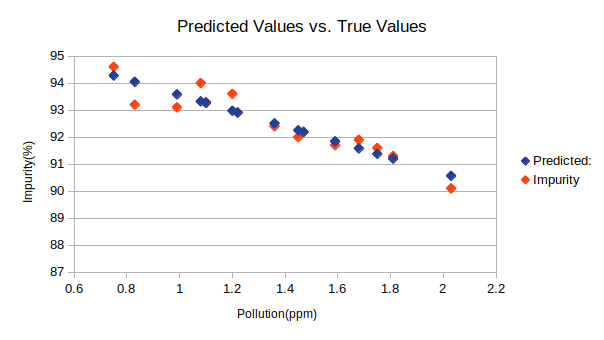
\includegraphics[scale=0.75]{9pred.png}
\end{center}
We see that the model fits well, as we would hope.
\end{enumerate}
\end{enumerate}
\end{document}
